
%\documentclass[gray,trans]{beamer} % com o mod transpar�ncia
%\documentclass[gray]{beamer}
\documentclass[trans,note]{beamer}

\usetheme{Madrid}

%\usetheme{Marburg} % Template ideial para SBMF
%\usetheme{CambridgeUS}
 %\usetheme{Boadilla}
%\usetheme{default}


%\usecolortheme{structure} 
%\usebeamercolor{structure}

% \usefonttheme[onlylarge]{structurebold}
% \usefonttheme{default}
% \setbeamerfont*{frametitle}{size=\normalsize,series=\bfseries}
 % \setbeamertemplate{navigation symbols}{}

% \usepackage[latin1]{inputenc} 
% \usepackage[brazil]{babel}
\usepackage[english]{babel}
\usepackage[latin1]{inputenc}

\usepackage{graphicx,url}
\usepackage{fancyhdr}

\usepackage{tikz}
\usetikzlibrary{arrows}
 \tikzstyle{block}=[draw opacity=0.3,line width=1.0cm]

% Class options include: notes, notesonly, handout, trans,
% hidesubsections, shadesubsections,
% inrow, blue, red, grey, brown

% Theme for beamer presentation.
%\usepackage{beamerthemeclassic}
% \usepackage{beamerthemebars}
% \usepackage{beamerthemesplit}
% \usepackage{beamerthemetree}
% \usepackage{beamerthemelined}

\title{Formal Modelling of \\ a Microcontroller Instruction Set in B}

%\subtitle{Qualifica��o de Mestrado} % Enter your title betweencurlybraces
\author{Val�rio Medeiros Jr, David D�harbe}
\institute{Federal University of Rio Grande do Norte} % Enter your institute name between curly braces
\date{20 August 2009} % Enter the date or \today between curly braces

\begin{document}

%% Keywords for the B method
\newcommand{\MACHINE}{\operatorname{\mathbf{MACHINE}}}
\newcommand{\REFINEMENT}{\operatorname{\mathbf{REFINEMENT}}}
\newcommand{\IMPLEMENTATION}{\operatorname{\mathbf{IMPLEMENTATION}}}
\newcommand{\REFINES}{\operatorname{\mathbf{REFINES}}}
\newcommand{\SEES}{\operatorname{\mathbf{SEES}}}
\newcommand{\INCLUDES}{\operatorname{\mathbf{INCLUDES}}}
\newcommand{\IMPORTS}{\operatorname{\mathbf{IMPORTS}}}
\newcommand{\SETS}{\operatorname{\mathbf{SETS}}}
\newcommand{\CONSTANTS}{\operatorname{\mathbf{CONSTANTS}}}
\newcommand{\PROPERTIES}{\operatorname{\mathbf{PROPERTIES}}}
\newcommand{\CONCRETE}{\operatorname{\mathbf{CONCRETE}}}
\newcommand{\VARIABLES}{\operatorname{\mathbf{VARIABLES}}}
\newcommand{\ASSERTIONS}{\operatorname{\mathbf{ASSERTIONS}}}
\newcommand{\CONCRETEVARIABLES}{\operatorname{\mathbf{CONCRETE\_VARIABLES}}}
\newcommand{\DEFINITIONS}{\operatorname{\mathbf{DEFINITIONS}}}
\newcommand{\VAR}{\operatorname{\mathbf{VAR}}}
\newcommand{\IN}{\operatorname{\mathbf{IN}}}
\newcommand{\INVARIANT}{\operatorname{\mathbf{INVARIANT}}}
\newcommand{\INITIALISATION}{\operatorname{\mathbf{INITIALISATION}}}
\newcommand{\OPERATIONS}{\operatorname{\mathbf{OPERATIONS}}}
\newcommand{\BEGIN}{\operatorname{\mathbf{BEGIN}}}
\newcommand{\END}{\operatorname{\mathbf{END}}}
\newcommand{\PRE}{\operatorname{\mathbf{PRE}}}
\newcommand{\IF}{\operatorname{\mathbf{IF}}}
\newcommand{\THEN}{\operatorname{\mathbf{THEN}}}
\newcommand{\ELSE}{\operatorname{\mathbf{ELSE}}}
\newcommand{\ELSIF}{\operatorname{\mathbf{ELSIF}}}
\newcommand{\ANY}{\operatorname{\mathbf{ANY}}}
\newcommand{\WHERE}{\operatorname{\mathbf{WHERE}}}
\newcommand{\CASE}{\operatorname{\mathbf{CASE}}}
\newcommand{\OF}{\operatorname{\mathbf{OF}}}
\newcommand{\EITHER}{\operatorname{\mathbf{EITHER}}}
\newcommand{\AND}{\operatorname{\mathbf{AND}}}
\newcommand{\OR}{\operatorname{\mathbf{OR}}}
\newcommand{\NOT}{\operatorname{\mathbf{NOT}}}
\newcommand{\WHILE}{\operatorname{\mathbf{WHILE}}}
\newcommand{\DO}{\operatorname{\mathbf{DO}}}
\newcommand{\VARIANT}{\operatorname{\mathbf{VARIANT}}}
\newcommand{\FALSE}{\operatorname{\mathbf{FALSE}}}
\newcommand{\TRUE}{\operatorname{\mathbf{TRUE}}}

%% Commonly used math entities
\newcommand{\pow}{\operatorname{\mathbb{P}}}
\newcommand{\nat}{\operatorname{\mathbb{N}}}
\newcommand{\pfun}{\operatorname{\rightarrow\mkern-22mu+}}
\newcommand{\fset}{\operatorname{\mathbb{F}}}
\newcommand{\dom}{\operatorname{\mbox{dom}}}
\newcommand{\ran}{\operatorname{\mbox{ran}}}
\newcommand{\natone}{\operatorname{\mathbb{N}_1}}
\newcommand{\integer}{\operatorname{\mathbb{Z}}}
\newcommand{\fun}{\operatorname{\rightarrow}}
\newcommand{\domr}{\operatorname{\triangleleft}}
\newcommand{\seq}{\operatorname{\mathbf{seq1}}}
\newcommand{\ovr}{\operatorname{\oplus}}
\newcommand{\BOOL}{\operatorname{\mathbf{BOOL}}}
\newcommand{\pred}{\operatorname{\mathbf{pred}}}
\newcommand{\Bsucc}{\operatorname{\mathbf{succ}}}


%\usepackage{supertabular}

% DEFINITION DES CARACTERES MATHEMATIQUES B
%------------------------------------------
\def\@setmcodes#1#2#3{{\count0=#1 \count1=#3
	\loop \global\mathcode\count0=\count1 \ifnum \count0<#2
	\advance\count0 by1 \advance\count1 by1 \repeat}}

%\@setmcodes{`A}{`Z}{"7441}
%\@setmcodes{`a}{`z}{"7461}

\mathcode`\;="8000 % Makes ; active in math mode
{\catcode`\;=\active \gdef;{\semicolon\;}}
\mathchardef\semicolon="003B
%    Nominal distance from top of paper to top of page
% \topmargin 0 pt
% \textheight 53\baselineskip
% 
% %   Left margin on odd-numbered pages
% \oddsidemargin  0.15 in
% %   Left margin on even-numbered pages
% \evensidemargin 0.35 in
% %   Width of marginal notes.
% \marginparwidth 1 in
% %   Note that \oddsidemargin = \evensidemargin
% \oddsidemargin 0.25 in
% \evensidemargin 0.25 in
% \marginparwidth 0.75 in
% \textwidth 5.875 in % Width of text line.
% 
% \setlength{\parindent}{0pt}
% \setlength{\parskip}{0ex}

% DEFINITION DES FONTS
%---------------------
% The AMS extra symbol fonts are loaded.
% Note: sometimes called euxm10
\font\msx=msam10
% Note: sometimes called euym10
\font\msy=msbm10

\newfam\msxfam \textfont\msxfam=\msx
\newfam\msyfam \textfont\msyfam=\msy

\def\famletter#1{\ifcase #1 0\or 1\or 2\or 3\or 4\or 5\or 6\or 7\or
	8\or 9\or A\or B\or C\or D\or E\or F\fi}

\edef\fx{\famletter\msxfam}
\edef\fy{\famletter\msyfam}

\def\bbold{\fam\msyfam \msy}

% SYMBOLES B
%-----------
% makes a quoted expression in mathematical text
\def\token#1{\hbox{`$#1$'}}
% used for error messages in Z specs
\def\report#1{\hbox{`{\tt #1}'}}

% \@myop makes an operator, with a strut to defeat TeX's vertical adjustment.
\def\@myop#1{\mathop{\mathstrut{#1}}\nolimits}

% This underscore doesn't have the little kern --- you get an italic
% correction anyway in math mode.
\def\_{\leavevmode \vbox{\hrule width0.5em}}

% Save \q as \xq for quantifiers q.
\let\xforall=\forall
\let\xexists=\exists
\let\xlambda=\lambda
\let\xmu=\mu

% \p and \f make arrows with 1 and 2 crossings resp.
\def\p#1{\mathrel{\ooalign{\hfil$\mapstochar\mkern 5mu$\hfil\cr$#1$}}}
\def\f#1{\mathrel{\ooalign{\hfil
	$\mapstochar\mkern 3mu\mapstochar\mkern 5mu$\hfil\cr$#1$}}}

\let\mc=\mathchardef

\def	\pow		{\mbox{${\cal P}$}}
\def	\po1		{\mbox{${\cal P}_1$}}
\let	\cross		\times
\def	\lambda		{\@myop{\xlambda}}
\def	\lnot		{\neg\;}
\def	\land		{\mathrel{\wedge}}
\def	\lor		{\mathrel{\vee}}
\let	\implies	\Rightarrow
\let	\iff		\Leftrightarrow
\def	\forall		{\@myop{\xforall}}
\def	\exists		{\@myop{\xexists}}
\def	\semi		{\mathrel{\comp}}
\def	\ssemi		{\mathbin{\rm ;}}
\let	\ensembleVide	\emptyset
\let	\rel		\leftrightarrow
\def	\dom		{\@myop{\sf dom}}
\def	\ran		{\@myop{\sf ran}}
\def	\id		{\@myop{\sf id}}
\def	\comp		{\mathbin{\raise
			0.6ex\hbox{\oalign{\hfil$\scriptscriptstyle
			\rm o$\hfil\cr\hfil$\scriptscriptstyle\rm 9$\hfil}}}}
\def	\para		{\mbox{$\mid\mid$}}
\mc	\dres		"2\fx43
\mc	\rres		"2\fx42
\def	\ndres		{\mathbin{{\dres} \llap{$-$}}}
\def	\nrres		{\mathbin{{\rres}\llap{$-$}}}
\def	\lover		{\vartriangleleft{ \llap{$-\!\!\!\!-\!$}}}
\def	\rover		{\mathbin{{\rres}\llap{$\!-\!\!\!-$}}}
\let	\fun		\rightarrow
\def	\pfun		{\p\fun}
\def	\pinj		{\p\inj}
\mc	\inj		"3\fx1A
\def	\psurj		{\p\surj}
\mc	\surj		"3\fx10
\def	\bij		{\surj\!\!\!\!\!\!\!\inj}
\def	\nat		{\mbox{${\cal N}$}}
\def	\na1		{\mbox{${\cal N}_1$}}
\def	\num		{\mbox{${\cal Z}$}}
\def	\int		{\mbox{${\cal Z}$}}
\def	\rat		{\mbox{${\cal Q}$}}
\def	\div		{\mathbin{\rm /}}
\def	\mod		{\mathbin{\bf mod}}
\def	\upto		{\mathbin{\ldotp\ldotp}}
\def	\finset		{\mbox{${\cal F}$}}
\def	\finse1		{\mbox{${\cal F}_1$}}
\def	\ffun		{\f\fun}
\def	\finj		{\f\inj}
\def	\seq		{\@myop{\rm seq}}
\def	\cat		{\mathbin{\raise 0.8ex\hbox{$\mathchar"2\fx61$}}}
\def	\sep		{\hspace*{.05in}}

\setcounter{secnumdepth}{0}
\setcounter{tocdepth}{0}

%-------------------%
% Debut du document %
%-------------------%





\beamertemplatefootpagenumber % Mostra o n�mero de p�ginas

% Creates title page of slide show using above information
\begin{frame}
   \titlepage  
  \begin{center} 
  Project: B2ASM\\
  Avaliable at http://code.google.com/p/b2asm\\
  
\includegraphics[width=.14\textwidth]{figures/ufrn.png} \ \ \ \ \ \ \ \ \ \ \ \ \ \ \ \ \ \ \ 
  
\includegraphics[width=.14\textwidth]{figures/anp.png}  \ \ \ \ \ \ \ \ \ \ \ \ \ \ \ \ \ \ \
   
\includegraphics[width=.12\textwidth]{figures/dimap.png}
  \end{center}
  
\end{frame}
\note{Initial Slide} % Add notes to yourself that will be displayed when
  % typeset with the notes or notesonly class options


%\section [Agenda]{Agenda}


% Creates table of contents slide incorporating
% all \section and \subsection commands
 \begin{frame}
  \frametitle{Summary}
  \tableofcontents
 \end{frame} 

% Mostra um slide com destaque a atual se��o, em cada mudan�a de se��o
\AtBeginSection[]
{
\begin{frame}
\frametitle{Summary}
\tableofcontents[currentsection]
\end{frame}
}

  
\section{Introduction}


\begin{frame}
\frametitle{Overview}  

\begin{itemize}[<+->]
  \item The B method supports the construction of safety systems
  \begin{itemize}
    \item Until the implementation model
    \item But the result of this translation is not guaranteed by formal means
    \item Then the transformation process can introduce small bugs\\
       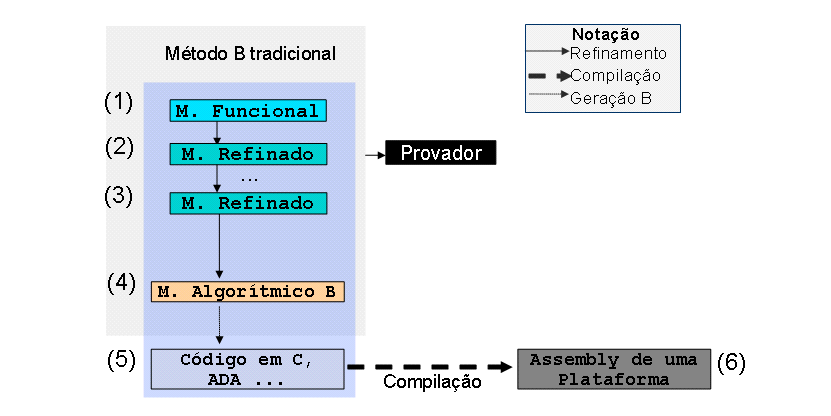
\includegraphics[width=.7\textwidth]{figures/passos_de_desenvolvimento_tradicional.png}
  \end{itemize}
  \item The last year a paper [Dantas, 2008] proposed a approach to extend the formal verification
  \item One key of this approach is the formal model of the instruction set  of execution platform % of such assembly languages
\end{itemize}
% TO-DO Ajustar a figura   

	\note{ ................... }
\end{frame}



\begin{frame}
\frametitle{Overview}  

\begin{itemize}[<+->]
  \item The B method supports the construction of safety systems
  \begin{itemize}
    \item Until the implementation model
    \item But the result of this translation is not guaranteed by formal means
    \item Then the transformation process can introduce small bugs\\
       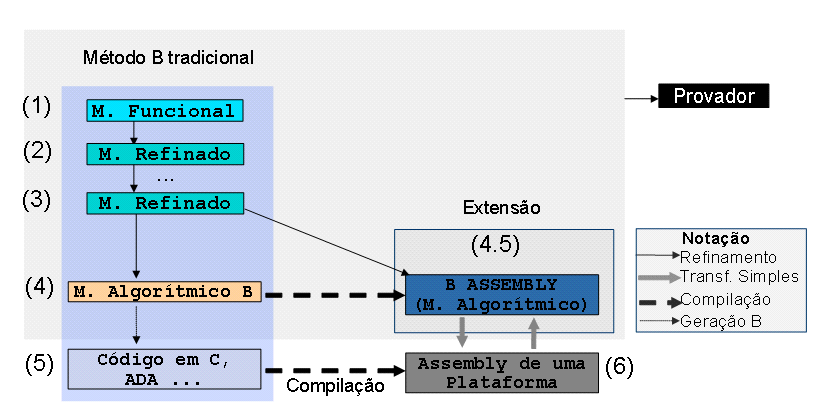
\includegraphics[width=.7\textwidth]{figures/passos_de_desenvolvimento_extendido.png}
  \end{itemize}
  \item The last year a paper [Dantas, 2008] proposed a approach to extend the formal verification
  \item One key of this approach is the formal model of the instruction set  of execution platform % of such assembly languages
\end{itemize}
% TO-DO Ajustar a figura

	\note{ ................... }
\end{frame}


\begin{frame}
\frametitle{Modelling}  

\begin{itemize}[<+->]
  \item The modelling is builded using some libraries developed
  \item The libraries has common concepts that can be used to others platforms too
  \item Utilities of this Formal Model:
  \begin{itemize}
    \item Documentation
    \item Simulation
    \item The formal verification until the assembly level
    \item A possible support to verify the Z80 design

  \end{itemize}
\end{itemize}

	\note{ ................... }
\end{frame}



\begin{frame}
\frametitle{Objective}  

\begin{itemize}[<+->]
  \item The main actual objective is represent the instruction set
    \begin{itemize}
    \item The aspects no-functional are not represented: logic circuits, pipeline, data bus, \ldots 
  \end{itemize}
  \item Because there are many efficient ways to verify hardware

\end{itemize}
% 

	\note{ ................... }
\end{frame}




%  % * Explain the cover of B Method 
%  % The solution is a framework proposed a paper [Dantas, 2009]
%  % The component key to this aproach is the formal model
%  % Then this paper gave u
% 
  \section{B Method}

\begin{frame}
\hypertarget{metodoB}{}
  \frametitle{B Method} 
  \begin{itemize}
    \item B method for software development is a formal method based on
	    \begin{itemize}
	    \item  B Abstract Machine Notation (AMN)
	    \item  First order logic, integer arithmetic and set theory
	    \end{itemize}
    \item Its constructions are very similar to those of the Z notation    
    \item Supports:
    \begin{itemize}
	    \item Modularization
	    \item Advanced techniques for proof development: user rules, parallelization, etc.
	    \item Refinements proved until basic constructs of programming language  
	    \item Code generator to programming language
	    \item \ldots
    \end{itemize}   
  \end{itemize}
\end{frame}
    
    
%     
% \begin{frame}
% \frametitle{B Method- Simple example}
% \begin{figure}
%   % \begin{small}
%   $$
%   \begin{array}{lcl}
%     \begin{array}[t]{l}
%       \MACHINE \\ \quad  \mathit{micro} \\
%       \SEES \\ \quad \mathit{TYPES}, \mathit{ALU} \\
%       \INCLUDES \\  \quad \mathit{MEMORY} \\
%       \VARIABLES \\ \quad    \mathit{pc}  \\
%       \INVARIANT \\ \quad \mathit{pc} \in \mathit{INSTRUCTION} 
%     \end{array}
%     & \hspace*{0cm} &
%     \begin{array}[t]{l}
%       \INITIALISATION  \mathit{pc} := 0 \\
%       \OPERATIONS\\
%       \mathit{JMP} \mathit{( jump )} = \\
%       \quad \PRE \mathit{jump} \in \mathit{INSTRUCTION}\\ 
%       \quad \THEN \mathit{pc} := \mathit{jump}\\  
%       \quad \END \\
%       \END
%     \end{array}
%   \end{array}
%   $$
% \caption{A very basic B machine.}
% \label{fig:maqB}
% \end{figure}
% \end{frame}
%  %  Basear-se nas notas escritas 
% 
  \section{Modelling the Instruction Set in B}
% \begin{frame}
%   \frametitle{Modelling  Microcontrollers}  
% 
%   \begin{itemize}[<+->]
%   \item Relations 
%   \begin{itemize}
%   	\item States of platform  $\Leftrightarrow$ States of modell
% 		\begin{itemize}
% 		\item Registers and Memory $\Leftrightarrow$  Variables of model
% 		\end{itemize}
% 	\item Assembly Instructions $\Leftrightarrow$ B operations
%         \begin{itemize}
%         \item Changes of states of platform $\Leftrightarrow$ B substitutions
%         \end{itemize}
%   \end{itemize}
%     
%  \end{itemize}
% \end{frame}


\begin{frame}
 \frametitle{Structure of B Projects}
 \begin{center}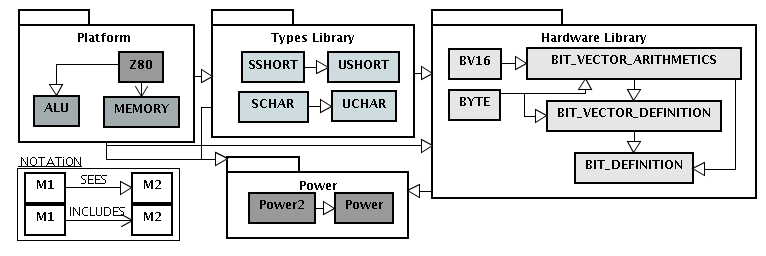
\includegraphics[width=1.\textwidth]{figures/diagramaEstrutural_vertical.png}
 \end{center}

 \end{frame}

 

 
\begin{frame}
 \frametitle{Hardware Library Project}

  	  	\begin{itemize}
 			\item The module \textit{BIT\_DEFINITION} has:
 			\begin{itemize}
                 
  	  		\item Definition of \textit{Bit}\\
  			{\small
 			$
 			\begin{array}{l}
 			\mathit{BIT} = 0..1 \\
 			\end{array}
 			$
 			}
 
 			\item The function $\mathit{bit\_not}$ is a unary function:
			{\small
			$
			\begin{array}{l}
			\mathit{bit\_not}  \in  \mathit{BIT}  \fun  \mathit{BIT}  \land \\
			\forall (\mathit{bb}).(\mathit{bb} \in \mathit{BIT} \implies \mathit{bit\_not}(\mathit{bb}) = 1-\mathit{bb})\\
			\end{array}
			$
			}

			\item Some utils lemmas to development proofs

			{\small
			$
			\begin{array}{l}
			\mathit{bit\_not}(0) = 1; 	\mathit{bit\_not}(1) = 0; \\
			\forall (\mathit{bb}).(\mathit{bb} \in \mathit{BIT} \implies \mathit{bit\_not}(\mathit{bit\_not}(\mathit{bb})) = \mathit{bb});
			\end{array}
			$
			}
			

			\end{itemize}
  		\end{itemize}


\end{frame}


 
 
\begin{frame}
 \frametitle{Hardware Library Project}

 	\begin{itemize}
 	  		\item The module \textit{BIT\_DEFINITION} also has:
 	  		\begin{itemize}
            \item The conjunction is a binary function defined as:
			{\small
			$
			\begin{array}{l}
			\mathit{bit\_and} \in \mathit{BIT} \times \mathit{BIT} \fun \mathit{BIT} \land \\
			\forall (\mathit{b1}, \mathit{b2}).(\mathit{b1}  \in \mathit{BIT}  \land \mathit{b2} \in \mathit{BIT} \implies \\
			\quad ((\mathit{bit\_and}(\mathit{b1}, \mathit{b2}) = 1) \iff (\mathit{b1} =1)  \land  (\mathit{b2} = 1))) \land \\
			 bit\_and(0,0) = 0	\land bit\_and(0,1) = 0	\land\\
			 bit\_and(1,0) = 0	\land bit\_and(1,1) = 1 \\
			\end{array}
			$
			}
 	  		\item Definions of 	$\mathit{bit\_or},\mathit{bit\_xor}$ and
 	  		$bool\_to\_bit$.
 	  		\item Lemmas for associativity and commutativity of functions
           \end{itemize}



           
 	\end{itemize}


\end{frame}


\begin{frame}
 \frametitle{Hardware Library Project}

 	\begin{itemize}
       \item  The module \textit{BIT\_VECTOR\_DEFINITION} has:

           \begin{itemize}
	 	  		\item Definition of bit vectors:
				{\small
				$
				\begin{array}{l}
				\mathit{BIT\_VECTOR} = \seq (\mathit{BIT}) % Implementa��o antiga, mas vale
				\end{array}
				$
				}
	 	  		\item Definition of functions:
	 	  		 {\small
	 	  		 	          
	          \it bv\_nat  $\in$  \it BIT\_VECTOR  $\fun$ $\nat$
	          $\land$ \\
	          \it bv\_nat \rm =  $\lambda$  \rm (\it bv\rm )\rm .\rm (\it bv 
	          $\in$  \it BIT\_VECTOR  $\mid$ \\ \rm (  $\sum$  \it idx \rm . \rm (\it idx  $\in$  \bf dom\rm (\it bv\rm )  $\mid$  \rm
	          (\rm 2$^{idx}$\rm )  $\times$  \it bv\rm (\it idx\rm )\rm )\rm )\rm )
			   
% 				$
% 				\begin{array}{l}
% 				\mathit{bv\_size} \in \mathit{BIT\_VECTOR} \fun \nat_1 \land \\
% 				\mathit{bv\_size} = \lambda bv \bullet (bv \in \mathit{BIT\_VECTOR} \mid \mathbf{size}(bv))
% 				\end{array}
% 				$
				}
				\item It has others functions: \textit{bv\_catenate}, \textit{bv\_sub},
				\textit{bv\_not}, \textit{bv\_and}, \textit{bv\_or}, \textit{bv\_xor},
				\textit{bv\_set}, \textit{bv\_clear} and \ldots
				\begin{itemize}
		                  \item These functions use the definitions of  \textit{BIT\_DEFINITION}
		              	\end{itemize}
	           \end{itemize}
		\item The module \textit{BIT\_VECTOR\_ARITHMETICS} define basics arithmetic functions
        \item The module \textit{BYTE} and \textit{BV16\_DEFINITION} define specialized functions for bit vectors of size 8 and 16
 	\end{itemize}

\end{frame}




\begin{frame}
 \frametitle{Types Library Project}
	  	\begin{itemize}
                    
	        \item Define the common types and functions on platforms of 8 and 16 bits
	        \item For example:
	        \begin{itemize}
	          \item Function: \it uchar\_schar $\in$ \it UCHAR $\fun$ \it SCHAR	  
				%\hspace*{0.0in} 
	%  		  \hspace*{0.0in}\it uchar\_schar\rm = $\lambda$ \rm (\it v1\rm )\rm .\rm (\it v1 $\in$ \it UCHAR
	%  			$\land$  \it v1 $\leq$ \it SCHAR\_MAX $\mid$  \it v1\rm )  $\land$\\
	%  			\hspace*{0.0in}\it uchar\_schar\rm = $\lambda$ \rm (\it v1\rm )\rm .\rm (\it v1 $\in$ \it UCHAR
	%  			$\land$   $\neg$ \rm (\it v1 $\leq$ \it SCHAR\_MAX\rm )  $\mid$  \it v1\rm -\it UCHAR\_MAX \rm + \rm 1
	%  			\rm )

	          \item Lemma: $\forall(x).( x \in UCHAR \Rightarrow
	          uchar\_schar(schar\_uchar(x)) = x)$
	        \end{itemize}
	      \end{itemize}
	
	\begin{table}[h]
	\begin{center}
	{\scriptsize
	\begin{tabular}{|c|c|c|c|c|c|c|}
	\hline
	 $Type$&$\mathit{UCHAR}$&$\mathit{SCHAR}$&$\mathit{USHORTINT}$&$\mathit{SSHORTINT}$&$\mathit{BYTE}$&$\mathit{BV16}$\\
	 \hline $Range$&0..255&-128..127&0..65.535&-32.768..32.767&--&--\\ \hline
	 $Size$ & 1 byte & 1 byte & 2 bytes & 2 bytes &  1 bytes & 2 bytes \\ \hline
	\end{tabular}
	}
	\end{center}
	\caption{Description of integer data types}
	\label{tab:types}
	\end{table}
\end{frame}

 
\begin{frame}
 \frametitle{Platform Project (Z80)}
  \begin{itemize}
    \item Z80 is a 8 bits microcontroller with 16 bits address space
    \item Supports:
    \begin{itemize}
      \item 158 instructions (included all of 8080 microcontroller )
      \item Several addressing modes and interruption types
      \item 256 input and output ports (8 bits)
      \item Some operations with 16 bits
    \end{itemize}

  
  \item Modelling 
  \begin{itemize}
  	\item States of platform  $\Leftrightarrow$ States of model
		\begin{itemize}
		\item Registers and Memory $\Leftrightarrow$  Variables of model
		\end{itemize}
	\item Assembly Instructions $\Leftrightarrow$ B operations
        \begin{itemize}
        \item Changes of states of platform $\Leftrightarrow$ B substitutions
        \end{itemize}
  
    
 \end{itemize}

      
  \end{itemize}

\end{frame}

\begin{frame}
\frametitle{Modelling Registers, Input/Output Ports and Instructions from Z80}
%  \begin{itemize}
%  \item Header of Modelling B
%  \end{itemize}  
	 {\scriptsize
	 \begin{sloppypar}
		\hspace*{.0in}\bf MACHINE\\
		\hspace*{.15in}\it Z80\\
		\hspace*{.0in}\bf INCLUDES\\
		\hspace*{.10in}\it MEMORY\\
		\hspace*{.0in}\bf SEES\\ \ldots
	% 	\hspace*{1.10in}\it ALU, \it BIT\_DEFINITION, \it BIT\_VECTOR\_DEFINITION,\\
	% 	\hspace*{1.10in}\it BYTE\_DEFINITION, \it BV16\_DEFINITION,\\
	% 	\hspace*{1.10in}\it UCHAR\_DEFINITION, \it SCHAR\_DEFINITION,\\
	% 	\hspace*{1.10in}\it SSHORT\_DEFINITION ,\it USHORT\_DEFINITION\\
		\end{sloppypar}
	}
% \begin{itemize}  
 %  \item The invariant:

	{\scriptsize
	\begin{sloppypar}
	\bf INVARIANT\\
	\hspace*{0.10in}\it rgs8  $\in$  \it id\_reg\_8  $\fun$  \it BYTE  $\land$ pc  $\in$  \it INSTRUCTION
	$\land$\\
	\hspace*{0.10in}\it  sp  $\in$  \it BV16  $\land$  \it ix  $\in$  \it BV16  $\land$  \it iy  $\in$  \it
	BV16  $\land$\\
	\hspace*{0.10in}\it i\_  $\in$  \it BYTE  $\land$  \it r\_ $\in$  \it BYTE  $\land$ iff1  $\in$  \it BIT
	$\land$ \it iff2  $\in$  \it BIT  $\land$ \\
	\hspace*{0.10in}\it im \rm $\in$ \rm (\it BIT $\times$ \it BIT\rm )  $\land$ \it i\_o\_ports  $\in$
	\it BYTE $\fun$  \it BYTE\\
	\ldots
	\end{sloppypar}
	
	}
	
%	\item A simple instruction
	{\scriptsize
	\begin{sloppypar}
    \bf OPERATIONS\\
	\hspace*{0.10in}\bf LD\_n\_A \rm ( \it nn \rm ) \rm =\\
	\hspace*{0.20in}\bf PRE \it nn $\in$ \it USHORT\hspace*{0.15in}\\ %$\land$  \it nn $\in$\it DATA\_R\_ADR
	\hspace*{0.20in}\bf THEN\\
	\hspace*{0.20in}\bf updateAddressMem \rm ( \it ushort\_to\_bv16 \rm ( \it nn \rm ) \rm , \it rgs8 \rm ( \it a0 \rm )
	\rm )  $\para$\\
	\hspace*{0.20in}\it pc \rm := \it instruction\_next \rm ( \it pc \rm )  $\para$  \it r\_ \rm := \it
	update\_refresh\_reg\rm (\it r\_\rm )\\
	\hspace*{0.10in}\bf END\rm\\
	\ldots
	\end{sloppypar}

	}

	%\end{itemize}
% \end{itemize}
% 	\begin{center}
% 	{\small
% 	$$
% 	\begin{array}{l}
% 	\mathit{BTFSS} (\mathit{ff}, \mathit{bb}) =\\
% 	\quad \PRE \mathit{ff} : \mathit{REGISTER} \land  \mathit{bb} : \mathit{BYTE\_INDEX} \\
% 	\quad \THEN \\
% 	\quad \quad	\IF \mathit{bitget}(\mathit{mem}(\mathit{ff}), \mathit{bb}) = 1 \THEN\\
% 	\quad\quad\quad	   \mathit{pc} :=\mathit{instruction\_next}(\mathit{instruction\_next}(\mathit{pc}))\\
% 	\quad\quad	\ELSE\\
% 	\quad\quad\quad	  \mathit{pc} := \mathit{instruction\_next}(\mathit{pc})\\
% 	\quad\quad	\END\\
% 	\quad \END
% 	\end{array}
% 	$$
% 	}\\
% 	Instru��o de controle do \textit{PIC16C432}
%
% 	\end{center}

\end{frame}

% 
%  \include{content/4_Description}
% 
  \section{Proof Process}

\begin{frame}
\frametitle{Proof Process of Projects}

\begin{itemize}
   \item Statistics:\\
    \begin{center}{\footnotesize
  	 \begin{tabular}{|c|c|c|c|}
		\hline
		 \textsl{Projects} &  \textsl{POs}	& \textsl{POs WD} &	\textsl{Total}\\
		\hline
		\textit{Power} & 	21 &	4 &	25\\
		\hline
		\textit{Types Library} &	22 &	68 &	90\\
		\hline
		\textit{Hardware Library} &	108 &	324 &	432\\
		\hline
		\textit{Z80} &	631	 & 2470 & 	3101\\
		\hline
		   &    &  & 		\textbf{3648}\\
		\hline
	 \end{tabular}
   }
	\end{center}

   \item  Approximately 25\% are not solved automatically
	\item Approximately 18 days are needed to make almost all the proofs using a monolithic computer
	\item Some proofs needed to be replayed when we make changes to the specification
	\item The proof's time can be reduced using advanced features
	
	
\end{itemize}

\end{frame}


\begin{frame}
\frametitle{Proof Process - Advanced Features}

	\begin{itemize}
	\item Parallel theorem prover with 3 dual core computers 
	\item Two simple examples of user pass from theorem prover
	
 		\begin{itemize}
 		   \item Specific:\\
 		  	 $Pattern( x , y : dom(bitget) )$ \\ $\& ff(0) \& dd \& eh(dom(bitget)) \& ss \& pr;$\\
 		    \ldots
 		   \item General:\\
 		   	$Pattern( x : dom(y) )$ \\ $\& ff(0) \& dd \& eh(dom(y)) \& ss \& pr;$
         \end{itemize}
        
    \end{itemize}
    
\end{frame}




%  % Example proof commands  
%  
%  \include{content/6_Related_works}
% 
   \section{Conclusions}





 \begin{frame}
 \frametitle{Considerations about the work}
    
 \begin{itemize}
   \item It can be used to: \ \ \ \ \ \ \ \ \ \ \ \ \ \ \ \ \ \ \ \ \ \ \ \ \ \ \ \ \ \ \ 
    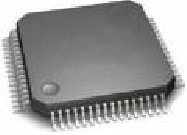
\includegraphics[width=.2\textwidth]{figures/processador_generico.jpg}
 	\begin{itemize} 
 	  \item Identifi��o de erros no manual ou projeto
 	  \item Important to  assembly programmers
 	  \item Formal verification until assembly language \\
 	   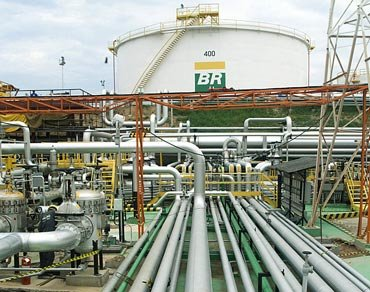
\includegraphics[height=.25\textheight]{figures/dutos.png} \ \ \ \ \ \ \ \ \ \ 
        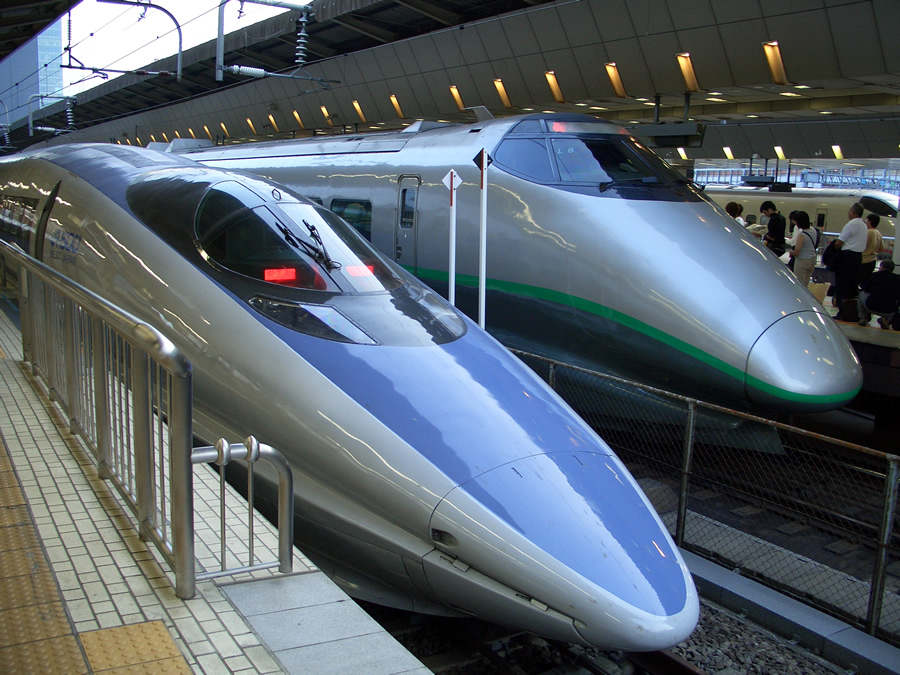
\includegraphics[height=.25\textheight]{figures/trem_bala2.png} 
 	\end{itemize} 
 \end{itemize} 
  	
 \end{frame}


\begin{frame}
  \frametitle{Sugestions/Doubts/Critics }
  	\begin{center}
    {\huge ?}\\
    
\includegraphics[width=.5\textwidth]{figures/rodin.png}\\
    \large{ If you prefer, my e-mail is 
    %\textcolor{blue!70!black}{\textit{valerio}}@ppgsc.ufrn.br or
    \textcolor{blue!70!black}{\textit{valerio.jr}}@gmail.com 
    }
	\end{center}
    
\end{frame}
% 

  
   



\end{document}